\chapter{Experimentation and design}



 \section{Modeling the short  pulse propagation}
    In order to have an easier understanding of the physical processes involved in the propagation of short pulses in a medium, it will be first necessary to focus on the dispersion that affects this medium. The purpose of this section is to consider the fiber as a linear optical medium while studying the pulse-propagation problem. Thus, it is possible to inspect the effect of GVD under certain circumstances where it dominates over the nonlinearities \citep{ AgrawalBook}. A further objective of this thesis is to implement a code capable of illustrating the Dispersion-induced broadening of optical pulses for both Gaussian and Hyperbolic-Secant (Sech) shapes.


    In this work, the normalized amplitude \emph{U} will be used and is obtained from  
  
            \begin{equation}\label{eq_A0}
                A(z,\tau ) = \sqrt{P_0}e^{\frac{-\alpha z}{2}} U(z,\tau) \ ,
            \end{equation}
            with
            \begin{equation}
                \tau =  \frac{T}{T_0} = \frac{t-z/v_g}{T_0} \ ,
            \end{equation}
        
        which is the time scale scaled to the input pulse width $T_0$.
        
        
        It is important to define relative lengths in order to understand the effect of the dispersion and/or nonlinearities on a pulse propagation
            \ \\
            \ \\
            \begin{equation}
                L_D = \frac{T^2_0}{|\beta_2|} \qquad and \qquad L_{NL} = \frac{1}{\gamma P_0} \ ,
            \end{equation}
        
        where $L_D$ is known as the dispersion length and $L_{NL}$ as the nonlinear length. Hence, the propagation of a pulse can present four different regimes depending on the length L of the fiber. This differentiation allows us to inspect the distinct phenomenon individually. Therefore, the students can comprehend how the pulse is affected by either the dispersion or the nonlinearities. The four regimes are 
        \begin{equation}
            \begin{aligned}\label{eq_lregimes}
               \mathbf{1} \quad L \ll L_D \quad & \quad L \ll  L_{NL} \ , \\
              \mathbf{2} \ \quad L \approx L_D \quad & \quad L \ll  L_{NL} \ , \\
               \mathbf{3} \quad L \ll L_D \quad & \quad L \approx  L_{NL} \ , \\
               \mathbf{4} \quad L \gg L_D \quad & \quad L \gg  L_{NL} \ . \\
            \end{aligned}
        \end{equation} 
        
        For the first case, both effects are negligible. In the second and third cases, the dispersion and nonlinearities act alone, respectively; and finally, both effects play an important role in the fourth case.
        
        \subsection{Modeling the effect of GVD}\label{subsect:gvd}
   
    
        
        Supposing a fiber length L such as $L \sim L_D$, $L << L_{NL}$, and setting $\gamma = 0$:  the equation \eqref{eq_nlse} becomes 
        
         \begin{equation}\label{eq_ugvd}
            \frac{\partial U}{\partial z} = -j\frac{\beta_2}{2}\frac{\partial^2U}{\partial T^2}.
        \end{equation}

        It is now necessary to define the incident field for the gaussian-like and the hyperbolic-Secant-like Pulses as 
            
        \begin{equation}\label{eq_u0t}
            U(0,T) = 
            \begin{cases}
                exp \left\{ -\frac{1+iC}{2} \left(\frac{T}{2T^2_0} \right)^{2m} \right\} \qquad \text{for Gaussian-shaped pulses}  \\
                \ \\
                sech\left( \frac{T}{T_0}\right) exp \left\{ -\frac{iCT^2}{2T^2_0} \right\} \qquad \text{for Hyperbolic-Secant pulses}.  \\
            \end{cases}
        \end{equation}
        
         Here are considered the initial chirp C for both types of pulses and the generalization for a supper-gaussian pulse, where m = 1 represents a chirped Gaussian pulse.
        
        
        Recalling the Fourier-transform method \eqref{eq_acft}, the equation \eqref{eq_ugvd} turns out to be the ordinary differential equation
        
        \begin{equation}\label{eq_ugvdw}
            i\frac{\partial\tilde{U}}{\partial z} = \frac{1}{2} \beta_2 \omega^2 \tilde{U} \ .
        \end{equation}
        
        Eventually, one can write the solution of the equation \eqref{eq_ugvdw} as
        
        \begin{equation}\label{eq_gvdufft}
            U(z,T) = FFT \left[ \tilde{U}(0,\omega) \ exp\{j\frac{\beta_2}{2}\omega^2z\} \right], 
        \end{equation}
        
        with
        
        \begin{equation}\label{eq_uw0gvd}
            \tilde{U}(0,\omega)  = FFT^{-1} \left[ U(0,T)\right] \ , 
        \end{equation}
        
        
        and its implementation in Python is straightforward regardless of the shape of the pulse.
        
        
        Agrawal et al. \citep{AgrawalBook} also propose a way to find the amplitude of a gaussian-shaped pulse at the point z by using 
        
        \begin{equation}\label{eq_ugvdg}
            U(z,T) = \frac{T_0}{(T^2_0 - i \beta z)^{1/2}} exp \left( -\frac{T^2}{2(T^2_0 - i \beta z)} \right) \ .
        \end{equation}
        
        This formula has fewer computational steps and was also added to the code to compare the results.  It is worth mentioning that the equation \eqref{eq_ugvdg} is only valid for unchirped  Gaussian pulses.
             
        Having these equations and using \href{https://numpy.org/}{Numpy}, was written a code to plot the pulse evolution. This code allows the user to change values like $\beta_2$ to see the dispersion-induced broadening. 
        
        \begin{figure}[label={fig:gvdmtp}, caption={Effect of GVD in a Gaussian pulse following Eq. \eqref{eq_ugvdg}.}]
        \centering
        \begin{tabular}[c]{cc}
        \centering
        \begin{subfigure}[b]{.53\textwidth}
		    \centering	
            \includegraphics[width=1\textwidth]{figures/chap3/gvdonlygaus.eps}
            \caption{Using Matplotlib and function \emph{Gaussian\_pulse\_GVD()} of the code.}\label{fig:gvdmtp1}
        \end{subfigure}
        \hfill
        \begin{subfigure}[b]{.53\textwidth}
		    \centering	
            \includegraphics[width=1\textwidth]{figures/chap3/gvdgausagr.png}
            \caption{Plot given in \citep{AgrawalBook} p. 68.}\label{fig:gvdmtp2}
        \end{subfigure}
        \end{tabular}
        \end{figure}
        
        
        \begin{figure}[label={fig:gvdmtps}, caption={Effect of GVD in a Gaussian (Fig. \subref{fig:gvdmtp3}) and in a Sech (Fig. \subref{fig:gvdmtp4}) pulse following Eq. \eqref{eq_gvdufft}, using Matplotlib and function \emph{incident\_field()} of the code.}]
        \centering
        \begin{tabular}[c]{cc}
        \centering
        \begin{subfigure}[b]{.53\textwidth}
		    \centering	
            \includegraphics[width=1\textwidth]{figures/chap3/gvdgaus.eps}
            \caption{Gaussian Pulse.}
            \label{fig:gvdmtp3}
        \end{subfigure}
        \hfill
        \begin{subfigure}[b]{.53\textwidth}
		    \centering	
            \includegraphics[width=1\textwidth]{figures/chap3/gvdsech.eps}
            \caption{Sech Pulse.}
            \label{fig:gvdmtp4}
        \end{subfigure}
        \end{tabular}
        \end{figure}
        
        \subsection{Modeling the effect of SPM}
        The next aspect to understand is the spectral broadening of a pulse because of nonlinear effects. In this case, the phenomenon of SPM influences under a propagation regime such as $ L_D \gg L \sim L_{NL} $, where $\beta_2=0$. The equation \eqref{eq_nlse} becomes: 
            \begin{equation}
                \frac{\partial U}{\partial z} = j\frac{e^{-\alpha z}}{L_{NL}}|U|^2 U \ ,
            \end{equation}
            %seite 98
            which phase shift can be defined as 
            \begin{equation} \label{eq_phi}
                \phi_{NL}(L,T) = |U(0,T)|^2 (L_{eff}/L_{NL})
            \end{equation}
            with 
            \begin{equation} \label{eq_leff}
                L_{eff} = \frac{1-e^{-\alpha L}}{\alpha} \ .
            \end{equation}
            
            If  $\alpha = 0$, then $L_{eff} = L$.
            
            That allow us to introduce the SPM-induced chirp as
            
            \begin{equation} \label{eq_spmchirp}
                \delta \omega(T) = -\frac{\partial \phi_{NL}}{\partial T} = -\left( \frac{L_{eff}}{L_{NL}} \right) \frac{\partial }{T} |U(0,T)|^2 \ ,
            \end{equation}
        
        
         and generalized for a super-Gaussian pulse:
            \begin{equation} \label{eq_spmchirpsg}
                \delta \omega(T) = \frac{2m L_{eff}}{T_0 L_{NL}}\left( \frac{T}{T_0}\right)^{2m-1}  exp\left\{ -\left( \frac{T}{T_0}\right)^{2m}   \right\}
            \end{equation}
        
        The code in Appendix \ref{sec:initvariables} uses the equations \eqref{eq_spmchirp} and \eqref{eq_spmchirpsg} for the Gaussian pulses. The integration can be carried using either the Euler's mid-point method \citep{euler} (function \emph{mid\_step(x0, f, T, *args)}), or the function cumtrapz\footnote{\href{https://docs.scipy.org/doc/scipy-0.14.0/reference/generated/scipy.integrate.cumtrapz.html}{Scipy documentation for 'cumtrapz'}}. For Hyperbolic-Secant pulses the process starts using the equation \eqref{eq_phi}, and its derivative gives as result the SPM-induced chirp. Figures \ref{fig:spmsg} and \ref{fig:spmsech} show the effect of SPM with $L_{eff} = L_{NL}$ \citep{AgrawalBook} on Gaussian and Sech pulses, respectively. The plots were made with Matplotlib and function \emph{incident\_field\_spm()} of the code.
        
        
        
        \begin{figure}[label={fig:spmsg}, caption={Effect of SPM in a Gaussian pulse. Following equations \eqref{eq_phi} - \eqref{eq_spmchirpsg}. }]
        \centering
        \begin{tabular}[c]{cc}
        \centering
        \begin{subfigure}[b]{.53\textwidth}
		    \centering	
            \includegraphics[width=1\textwidth]{figures/chap3/shift.eps}
            \caption{Phase shift $\phi_{NL}$.}
            \label{fig:shift_s}
        \end{subfigure}
        \hfill
        \begin{subfigure}[b]{.53\textwidth}
		    \centering	
            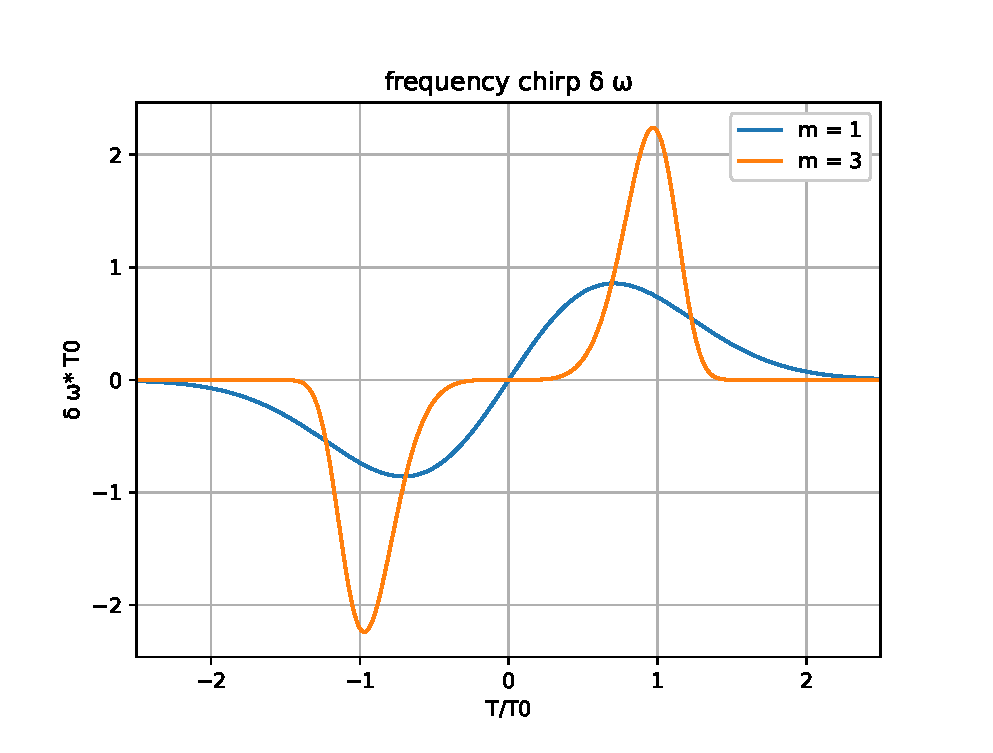
\includegraphics[width=1\textwidth]{figures/chap3/chirp.eps}
            \caption{Frequency chirp $\delta \omega$.}
            \label{fig:chirp_s}
        \end{subfigure}
        \end{tabular}
        \end{figure}
        
         \begin{figure}[label={fig:spmsech}, caption={Effect of SPM in a Sech pulse.}]
         \centering
        \begin{tabular}[c]{cc}
        \centering
        \begin{subfigure}[b]{.53\textwidth}
		    \centering	
            \includegraphics[width=1\textwidth]{figures/chap3/shift_sech.eps}
            \caption{Phase shift $\phi_{NL}$.}
            \label{fig:shift}
        \end{subfigure}
        \hfill
        \begin{subfigure}[b]{.53\textwidth}
		    \centering	
            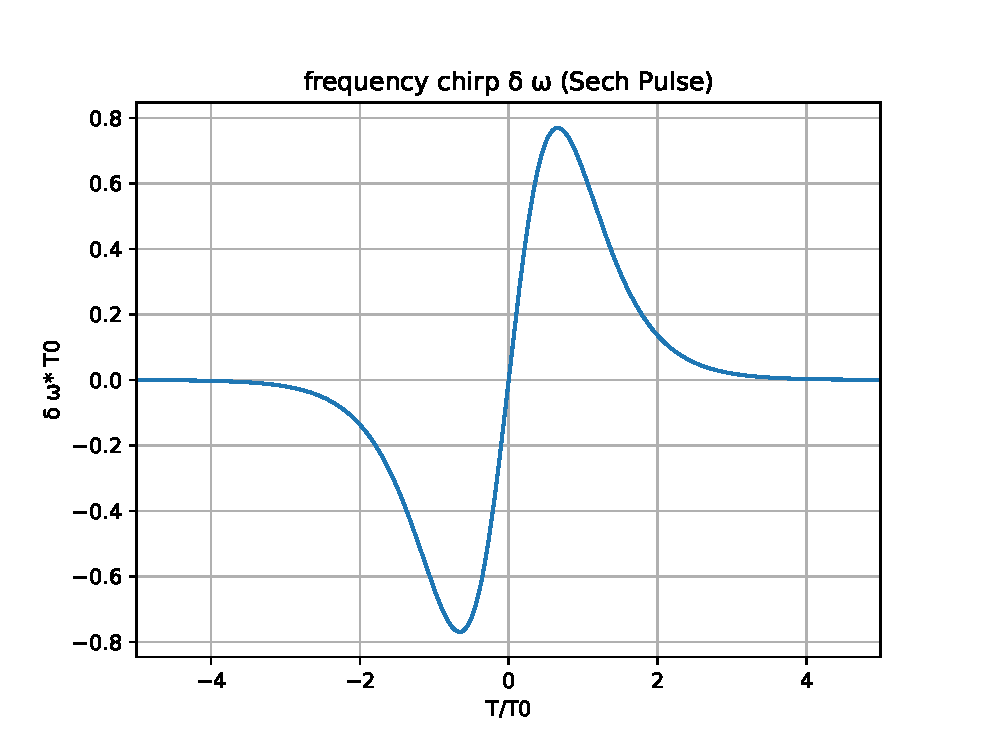
\includegraphics[width=1\textwidth]{figures/chap3/chirp_sech.eps}
            \caption{Frequency chirp $\delta \omega$.}
            \label{fig:chirp}
        \end{subfigure}
        \end{tabular}
        \end{figure}
        
        \subsection{Solution of the NLSE (SSFM)}\label{subsec:nlse}
            To initially solve the NLSE through the SSFM, the equations to follow are \eqref{eq_dpn}, \eqref{eq_dhat}, and \eqref{eq_nhat}. As the objective of this project is to create an interactive web tool with learning purposes, we avoided some calculations related to Raman Scattering and other nonlinear effects. Thus, equation \eqref{eq_nhat} turns out to be 
            \begin{equation} \label{eq_nhat2}
             \hat{\mathcal{N}} = i \left( 
             %\frac{e^{-\alpha z} \gamma P_0 T^2_0}{\left|\beta_2\right|} \left|U\right|^2 
             e^{-\alpha z} \gamma P_0 \left|U\right|^2 
             \right) \ ,
        \end{equation}
        
        and using equation \eqref{eq_A0} in \eqref{eq_dpn}, we obtain
        \begin{equation}\label{eq_dpn2}
            \frac{\partial U}{\partial z} = \left( \hat{\mathcal{D}} + \hat{\mathcal{N}} \right) U \ . 
        \end{equation}
        
        Here comes the symmetric SSFM of Equation \eqref{eq_azh2}. After running the calculation of the first $h/2$ section, one can implement the \emph{solve\_ivp()} function of Scipy\footnote{\href{https://docs.scipy.org/doc/scipy/reference/generated/scipy.integrate.solve_ivp.html}{Scipy documentation}}. The method used is the Explicit Runge-Kutta method of order 3(2), \emph{'RK23'}, as integration scheme and afterwards comes the next $h/2$ segment with the dispersion. The result is sampled and stored on both time and frequency domains. 
        
        It is now reasonable to introduce the parameter N, whose integer values give the soliton order:
        
        \begin{equation}\label{eq_n}
            N^2 = \frac{L_D}{L_{NL}} = \frac{\gamma P_0 T^2_0 \ . }{\left|\beta_2\right|}
        \end{equation}
        
        
        Depending on the value of \emph{N}, the SPM or GVD effects are more significant through the fiber. Some examples are carried by Agrawal \citep{AgrawalBook} for N = 0 (No SPM) and N = 1, then we compared them against the results we obtained with our code (figures \ref{fig:n1pb} and \ref{fig:n1nb}). The outcome is an evolution of the shape pulses, and the optical spectra appearing to be the same as those given in \citep{AgrawalBook}. Even though further experiments can grant a verification of the model.
        
         \begin{figure}[label={fig:n1pb}, caption={Solution of the NLSE using SSFM for N=1 and $\beta_2 > 0$.}]
         \centering	
         \begin{tabular}[c]{cc}
         \centering	
        \begin{subfigure}[b]{.53\textwidth}
        \centering	
            \includegraphics[width=1\textwidth]{figures/chap3/SSFM/eN1bt.eps}
            \caption{Envelope (time).}
            \label{fig:eN1bt}
        \end{subfigure}
        \begin{subfigure}[b]{.53\textwidth}
		    \centering	
            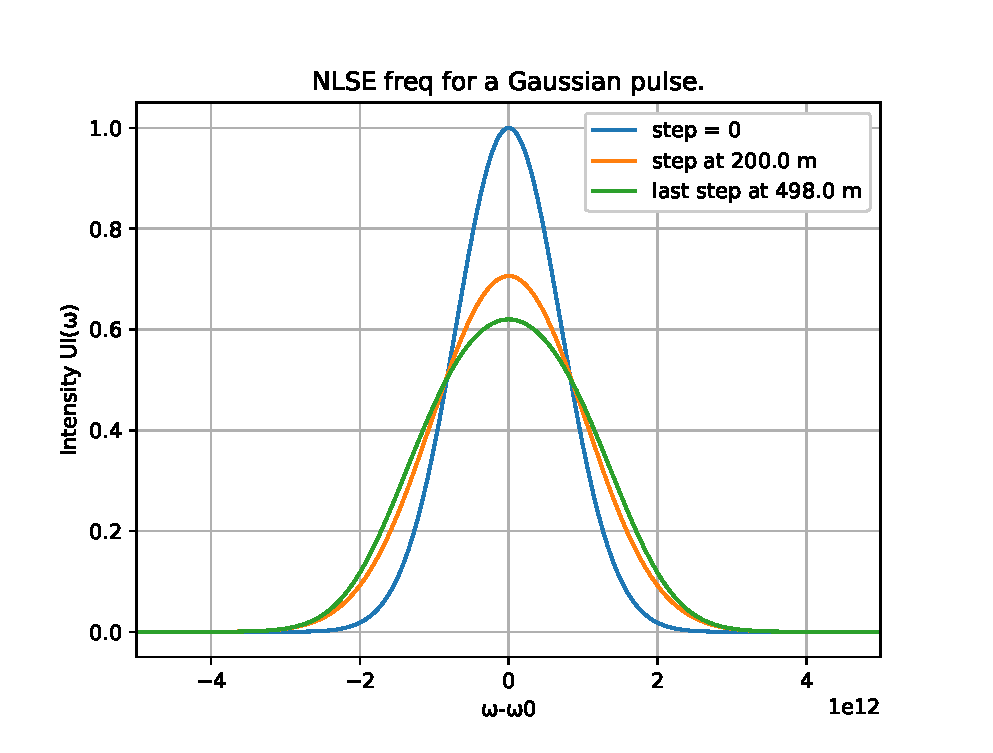
\includegraphics[width=1\textwidth]{figures/chap3/SSFM/eN1bs.eps}
            \caption{Envelope (spectrum).}
            \label{fig:eN1bs}
        \end{subfigure}
        \end{tabular}
        \begin{tabular}[c]{cc}
        \centering	
        \begin{subfigure}[b]{.53\textwidth}
		    \centering	
            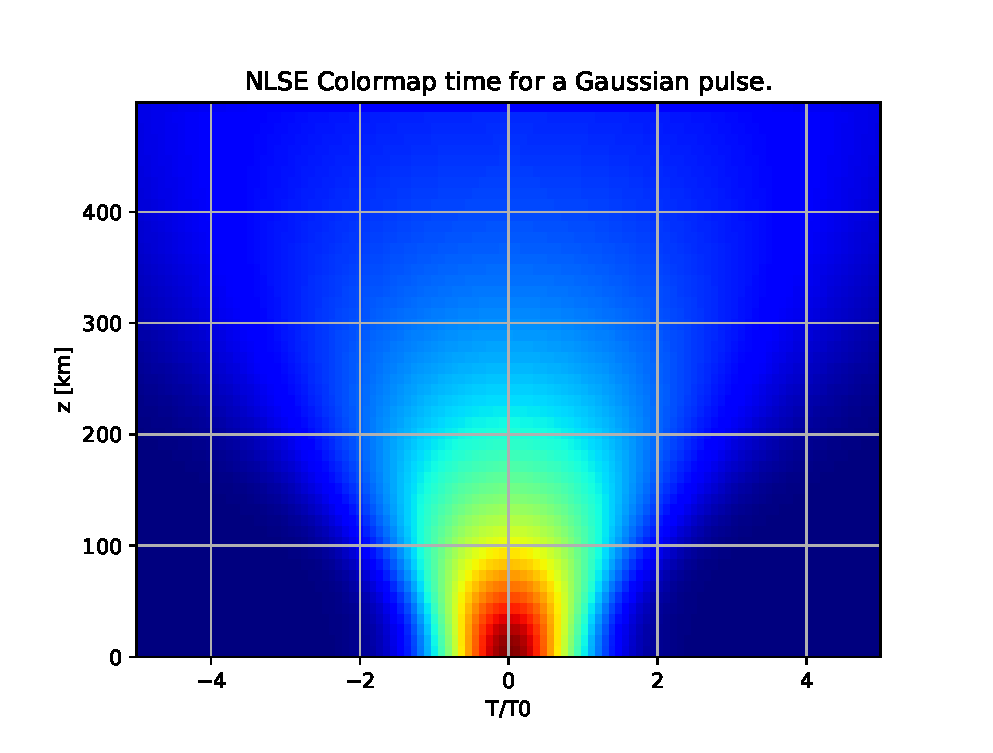
\includegraphics[width=1\textwidth]{figures/chap3/SSFM/N1bt.eps}
            \caption{Propagation (time).}
            \label{fig:N1bt}
        \end{subfigure}
        \hfill
        \begin{subfigure}[b]{.53\textwidth}
		    \centering	
            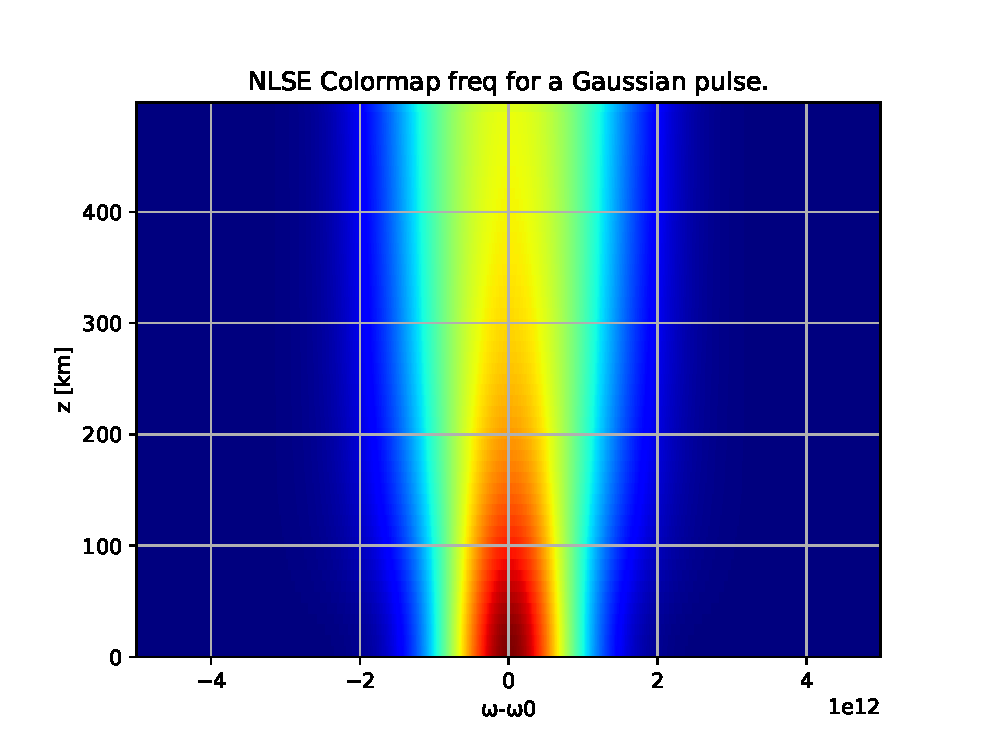
\includegraphics[width=1\textwidth]{figures/chap3/SSFM/N1bs.eps}
            \caption{Propagation (spectrum).}
            \label{fig:N1bs}
        \end{subfigure}
        \end{tabular}
        \end{figure}
        
         \begin{figure}[label={fig:n1nb}, caption={Solution of the NLSE using SSFM for N=1 and $\beta_2 < 0$.}]
         \centering	
         \begin{tabular}[c]{cc}
         \centering	
        \begin{subfigure}[b]{.53\textwidth}
		    \centering	
            \includegraphics[width=1\linewidth]{figures/chap3/SSFM/eN1nbt.eps}
            \caption{Envelope (time).}
            \label{fig:eN1nbt}
        \end{subfigure}
        \hfill
        \begin{subfigure}[b]{.53\textwidth}
		    \centering	
            \includegraphics[width=1\linewidth]{figures/chap3/SSFM/eN1nbs.eps}
            \caption{Envelope (spectrum).}
            \label{fig:eN1nbs}
        \end{subfigure}
        \end{tabular}
        \begin{tabular}[c]{cc}
        \centering	
        \begin{subfigure}[b]{.53\textwidth}
		    \centering	
            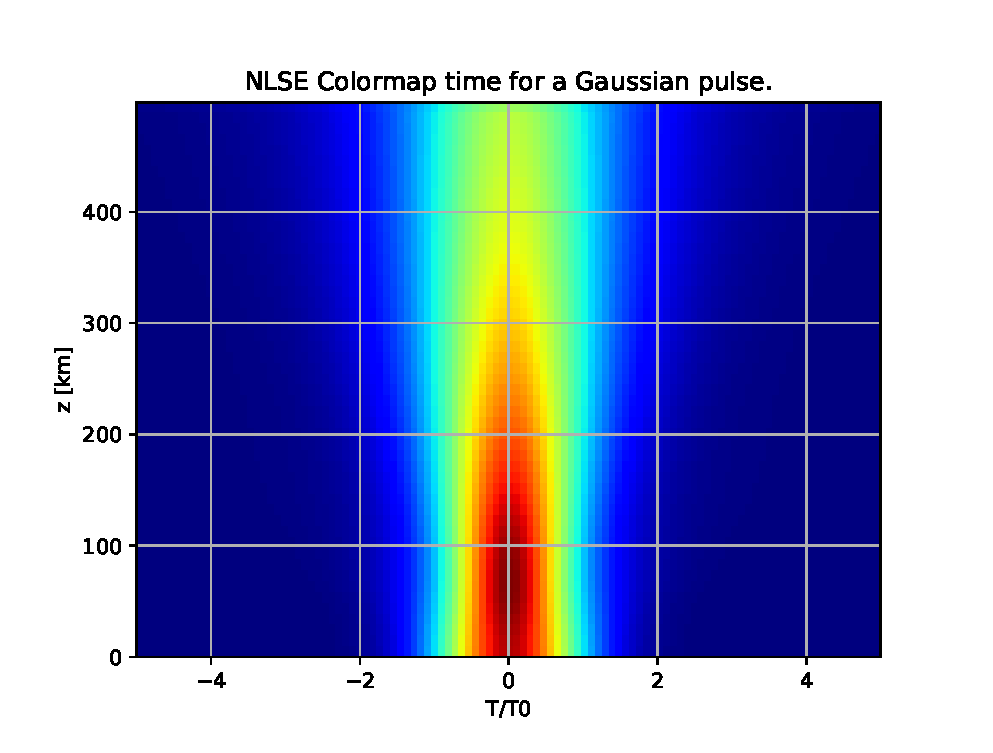
\includegraphics[width=1\linewidth]{figures/chap3/SSFM/N1nbt.eps}
            \caption{Propagation (time).}
            \label{fig:N1nbt}
        \end{subfigure}
        \hfill
        \begin{subfigure}[b]{.53\textwidth}
		    \centering	
            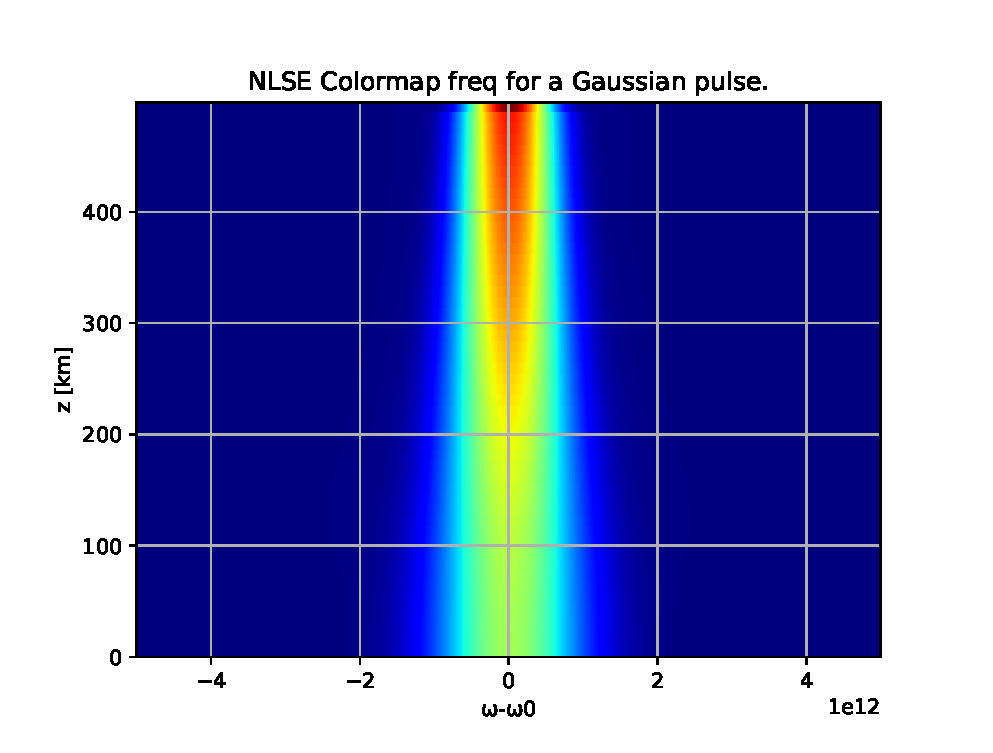
\includegraphics[width=1\linewidth]{figures/chap3/SSFM/N1nbs.eps}
            \caption{Propagation (spectrum).}
            \label{fig:N1nbs}
        \end{subfigure}
        \end{tabular}
        \end{figure}

    Following \citep{stolen}, the frequency spectra of a Gaussian pulse dependent on some values of maximum phase-shift is expected to be as given in figure \ref{fig:spmstol}. Figures \ref{fig:spm0pi}-\ref{fig:spm35pi} present the result of the function \emph{split\_step()} in the absence of dispersive effects (or close to the zero-dispersion region). The results of the code are very close to such shapes expected to get. The calculations were carried for a pulse $T_0 = 1ps$ in a lossless fiber with a length $L = 500m$, and $h = 0.004*L$ (250 steps).
    
     \begin{figure}[label={fig:spmssfm}, caption={Shape of the spectra for Gaussian pulses by maximum phase shift ($\phi_{NL}$).}]
         \centering	
         \begin{tabular}[c]{cc}
         \centering	
        \begin{subfigure}[b]{.53\textwidth}
		    \centering	
            \includegraphics[width=1\linewidth]{figures/chap3/ssfm_spm/stolen_SPM.png}
            \caption{Calculated freq. spectra. Taken from \citep{stolen}}
            \label{fig:spmstol}
        \end{subfigure}
        \hfill
        \begin{subfigure}[b]{.53\textwidth}
		    \centering	
            \includegraphics[width=1\linewidth]{figures/chap3/ssfm_spm/0pi.eps}
            \caption{$\phi_{NLmax}= 0$.}
            \label{fig:spm0pi}
        \end{subfigure}
        \end{tabular}
        \begin{tabular}[c]{cc}
        \begin{subfigure}[b]{.53\textwidth}
		    \centering	
            \includegraphics[width=1\linewidth]{figures/chap3/ssfm_spm/0_5pi.eps}
            \caption{$\phi_{NLmax}= 0.5\pi$.}
            \label{fig:spm05pi}
        \end{subfigure}
        \hfill
        \begin{subfigure}[b]{.53\textwidth}
		    \centering	
            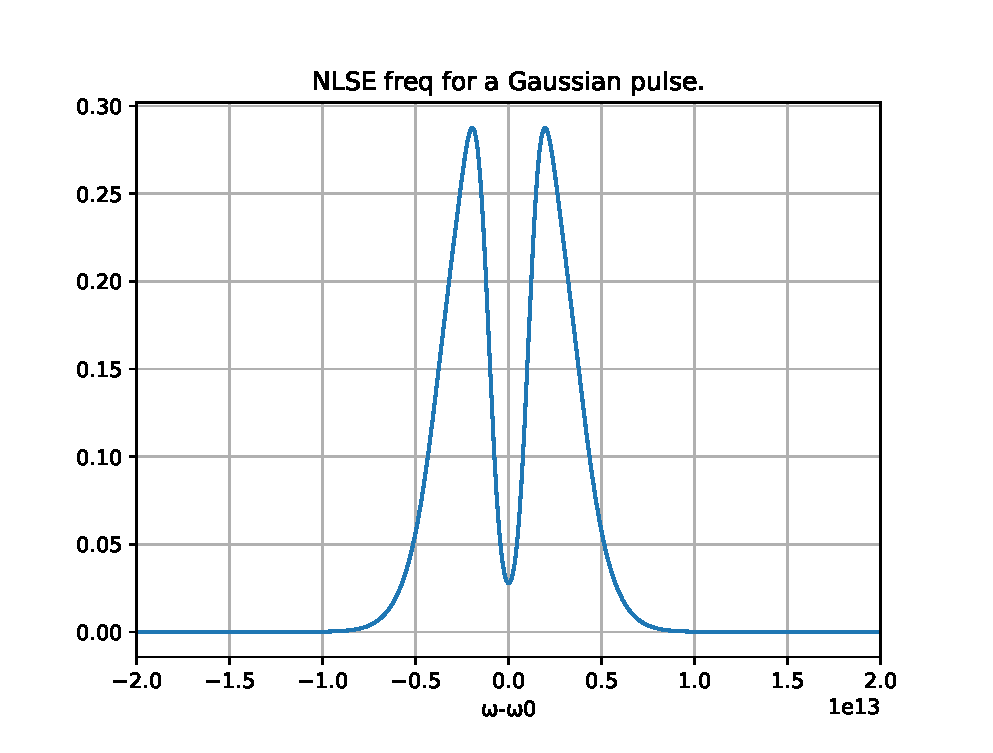
\includegraphics[width=1\linewidth]{figures/chap3/ssfm_spm/1_5pi.eps}
            \caption{$\phi_{NLmax}= 1.5\pi$.}
            \label{fig:spm15pi}
        \end{subfigure}
        \end{tabular}
        \begin{tabular}[c]{cc}
        \centering	
        \begin{subfigure}[b]{.53\textwidth}
		    \centering	
            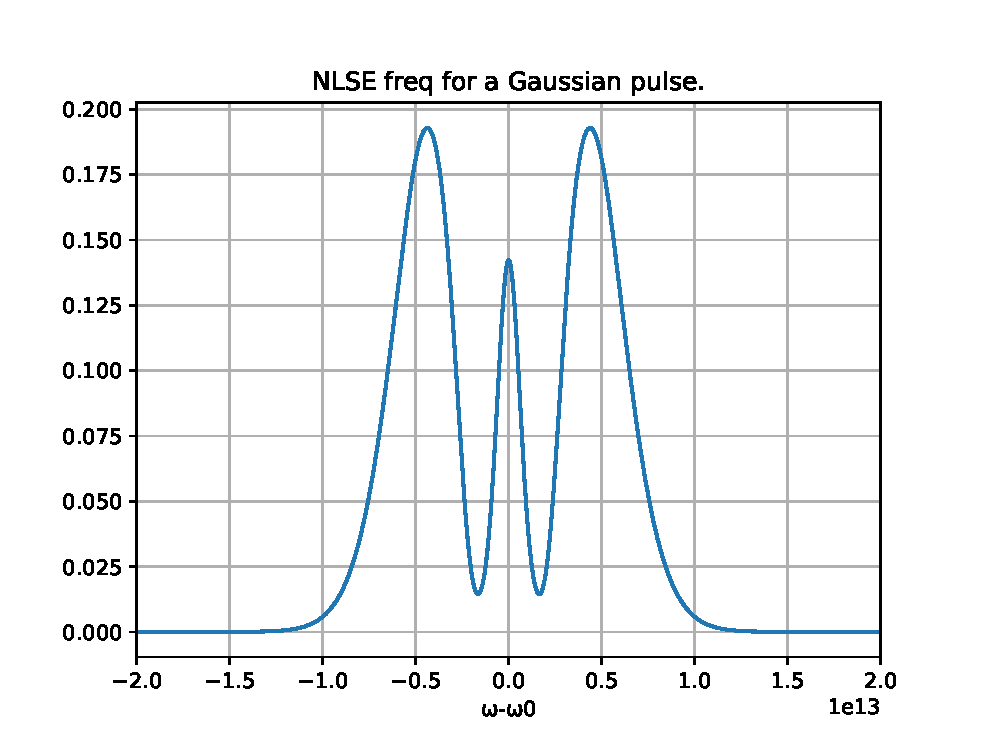
\includegraphics[width=1\linewidth]{figures/chap3/ssfm_spm/2_5pi.eps}
            \caption{$\phi_{NLmax}= 2.5\pi$.}
            \label{fig:spm25pi}
        \end{subfigure}
        \hfill
        \begin{subfigure}[b]{.53\textwidth}
		    \centering	
            \includegraphics[width=1\linewidth]{figures/chap3/ssfm_spm/3_5pi.eps}
            \caption{$\phi_{NLmax}= 3.5\pi$.}
            \label{fig:spm35pi}
        \end{subfigure}
        \end{tabular}
        \end{figure}
    
    
    
\section{Web-Tool}
    Following the experience with the Fiber-mode App (previous chapter), Dash/Plotly works as a framework to build the web interface for the code written in Python. Other options such as Bokeh\footnote{\url{https://bokeh.org/}}  were considered, even though Dash did not present problems with some of the types of data used. In addition, it allows us to present intuitive and cleaner plots. 
    
    This open-source Python library has the advantage of providing a reactive app, which will allow the students (or general users) to use it on browsers regardless of the device and operative system, i.e., smartphones (Android, IOS, etc.), tablets, computers, etc. Thus, we implement the theories of interactive learning and strive to provide an online tool (additional to the lectures, books, and illustrations) to aid the students and, expectedly, motivate them to understand the effects involved in the propagation of short pulses on fibers. 
    The purpose of deploying this additional content online is to reach the necessities of most of the target population. Last year several universities around the globe had to do online teaching, and many activities of students' life migrated to the online aspect \citep{Hassel2020}. The average students possess (now more than ever) access to the internet, and, additionally, most of them have experience using online apps. Now, one can say that the app is accessible and flexible due to the previously mentioned characteristics. However, the intuitive part comes while developing the user interface. The application should help the user learn from it without vast information or 'how-to' tutorials. Consequently, it is crucial to place elements like buttons, sliders, or plots correctly. Figure \ref{fig:appdash} shows the global structure of the code. 
    
    \begin{figure}[label={fig:appdash}, caption={Global structure of the code.}]
          %  \caption*{Source: Some Source}
        	\includegraphics[trim = 0cm 0.5cm 0 1.2cm, clip, width=0.75\textwidth]{figures/chap3/Apps.eps} 
        \end{figure}
    
     The file init\_variables.py (Appendix \ref{sec:initvariables}) contains the necessary classes and functions to run all calculations needed for either the page or a local use with Matplotlib or directly Dash as localhost. Figure \ref{fig:UML} presents the class diagram of this file. 

    As inputs for the class Pulse, we have the pulse width T0, the time window T, the pulse type (either 'Gaussian' or 'Sech'), the initial chirp \textbf{C}, and, if necessary, the value of \textbf{m} for Super-Gaussian pulses. This class is in charge of initializing the pulse at z = 0. Then, the class Propagation receives the required inputs to solve the problem needed, i.e., it can return the solution for just GVD effects, just SPM effects (in this case, the phase shift and the frequency chirp), or the SSFM. One can also calculate the values of $L_D$, $L_{NL}$, $L_{eff}$, and $\phi_{NLmax}$. It is possible further to create Plotly's graphical objects essential to plot with Dash. This way, one can avoid writing more code lines while building the dash apps. 
    
    \begin{figure}[label={fig:UML}, caption={Class Diagram of init\_variables.py}]	\includegraphics[width=.6\textwidth]{figures/chap3/init_variables.eps} 
        \end{figure}
    
    \subsection{GVD code for python}
    The code responsible for providing the app for only dispersive effects to the user is the file \emph{gvd.py} (Appendix B). This code uses either 'only\_gvd' or 'gauss\_gvd' as solution type. The class is then in charge of using the methods previously mentioned in section \ref{subsect:gvd}. Sliders allow changing  the values of $\beta_2$, initial chirp, m, and z, while a switch changes between Gaussian and Sech. In addition, the callbacks are always returning the actual state of the values along with the new calculated plots.  A simple block diagram of this page is presented in figure \ref{fig:gvddash}.
        
    \begin{figure}[label={fig:gvddash}, caption={Simplified Block-Diagram of gvd.py}]
          %  \caption*{Source: Some Source}
        	\includegraphics[trim = 2.5cm 12.5cm 5cm 2.5cm, clip, clip,width=1\textwidth]{figures/chap3/GVD.eps} 
        \end{figure}
    \subsection{SPM code for python}
    Figure \ref{fig:spmdash} bestows a simplified view of the SPM-page's structure.  The front-end receives values of $\gamma$, $P_0$, and m. Then, it shows the plots of phase shift and frequency chirp together with the actual value of $L_{NL}$. 
        \begin{figure}[label={fig:spmdash}, caption={Simplified Block-Diagram of spm.py}]
          %  \caption*{Source: Some Source}
        	\includegraphics[trim = 0.5cm 12.5cm 6.5cm 1.2cm, clip, clip,width=1\textwidth]{figures/chap3/SPM.eps} 
        \end{figure}
        
    \subsection{NLSE}
        As discussed in section \ref{subsec:nlse}, the SSFM plays a meaningful role in this app.  This page is more intricate than the previous two mentioned due to the complexity of its callbacks and the number of input variables. Again, its block diagram is in figure \ref{fig:ssfmdash}. 
        
        \begin{figure}[label={fig:ssfmdash}, caption={Simplified Block-Diagram of nlse.py}]
          %  \caption*{Source: Some Source}
        	\includegraphics[trim = 0.5cm 12.5cm 6.5cm 0.6cm, clip, clip,width=1\textwidth]{figures/chap3/SSFM.eps} 
        \end{figure}